%********************************************************************
% Appendix
%*******************************************************
% If problems with the headers: get headings in appendix etc. right
%\markboth{\spacedlowsmallcaps{Appendix}}{\spacedlowsmallcaps{Appendix}}
\chapter{Appendix to AtomicOrchid implementation}


\section{System architecture}
\begin{figure}[H]
  \centering
  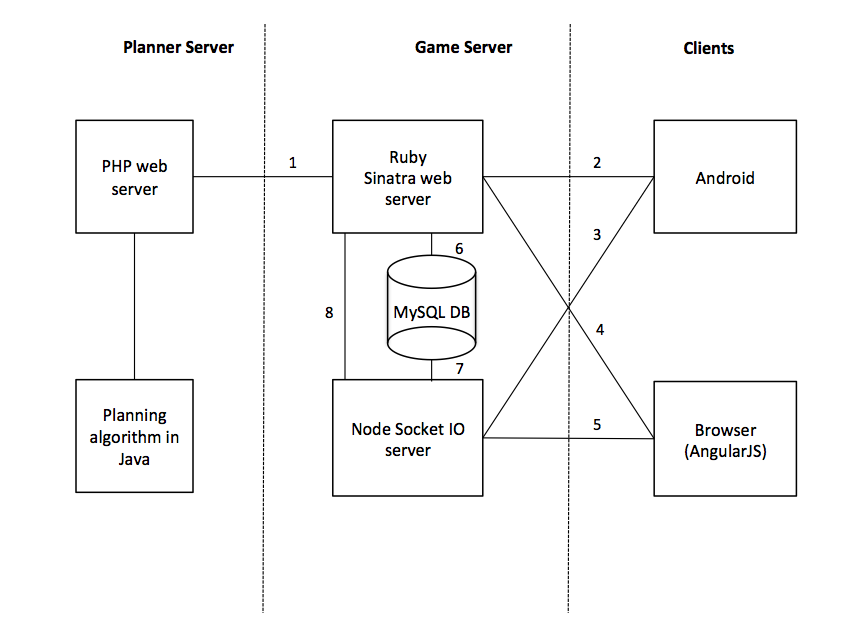
\includegraphics[width=1\textwidth]{img/Appendix/SystemDescription}
  \caption{Technological illustration of AtomicOrchid}
  \label{fig:systemDescription}
\end{figure}

\begin{table}[H]
\centering
\footnotesize
\begin{tabular}{|l|l|l|}
\hline
{\bf Interactions} & {\bf Compoents}                                                                                        & {\bf Descriptions}                                                                                                                                                                                                \\ \hline
1                  & \begin{tabular}[c]{@{}l@{}}Agent PHP server \\ \textless-\textgreater \\ Ruby game server\end{tabular} & \begin{tabular}[c]{@{}l@{}}1. game server requests to initialise planner \\ for a particular game session.\\ 2. game server requests to a plan to be\\ computed with a game status attached.\end{tabular}         \\ \hline
2                  & \begin{tabular}[c]{@{}l@{}}Android Client \\ \textless-\textgreater \\ Ruby server\end{tabular}        & \begin{tabular}[c]{@{}l@{}}1. Android client requests to join a game session\\ 2. Android requests game setup info\end{tabular}                                                                                   \\ \hline
3                  & \begin{tabular}[c]{@{}l@{}}Android Client \\ \textless-\textgreater \\ Node server\end{tabular}        & \begin{tabular}[c]{@{}l@{}}1. Android reports GPS updates, player feedbacks\\ chat messages.\\ 2. Node server transmit updates of player health\\ , target/player locations, messages, instructions.\end{tabular} \\ \hline
4                  & \begin{tabular}[c]{@{}l@{}}Ruby game server \\ \textless-\textgreater \\ Browser\end{tabular}          & \begin{tabular}[c]{@{}l@{}}1. Browser requests game setup info\\ 3. Node server transmit updates of player health\\ , target/player locations, messages, instructions.\end{tabular}                               \\ \hline
5                  & \begin{tabular}[c]{@{}l@{}}Node server \\ \textless-\textgreater \\ Browser\end{tabular}               & \begin{tabular}[c]{@{}l@{}}1. Browser reports plan edits and chat messages\\ 2. Node server transmit updates of player health\\ , target/player locations, messages, instructions.\end{tabular}                   \\ \hline
6                  & \begin{tabular}[c]{@{}l@{}}DB \\ \textless-\textgreater \\ Ruby server\end{tabular}                    & Rudy server retrieves and updates game status                                                                                                                                                                     \\ \hline
7                  & \begin{tabular}[c]{@{}l@{}}DB \\ \textless-\textgreater \\ Node server\end{tabular}                    & Node server retrieves and updates game status                                                                                                                                                                     \\ \hline
8                  & \begin{tabular}[c]{@{}l@{}}Ruby server \\ \textless-\textgreater \\ Agent PHP server\end{tabular}      & \begin{tabular}[c]{@{}l@{}}Rudy server requests Node server to push\\ latest status updates to clients \\ including player health, cloud status\\ target/player locations, messages, instructions\end{tabular}    \\ \hline
\end{tabular}
\caption{Communications between components}
\end{table}

\begin{figure}[H]
  \centering
  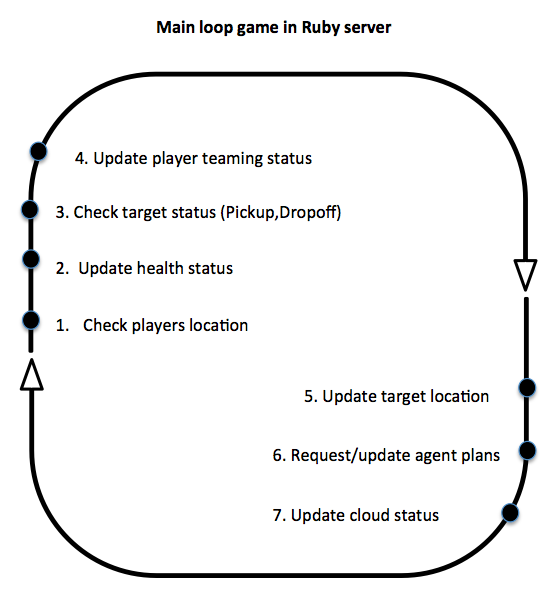
\includegraphics[width=1\textwidth]{img/Appendix/Mainloop}
  \caption{Handling of Game logic in Ruby server}
\end{figure}

\section{Data model}
\begin{table}[H]
\centering
\footnotesize
\begin{tabular}{llll}
\hline
{\bf Models}                        & {\bf Properties}                                                                                                                                                                                                       & {\bf Associations}                                                                                                                                  & {\bf Descriptions}                                                                                                               \\ \hline
\multicolumn{1}{|l|}{Game}         & \multicolumn{1}{l|}{\begin{tabular}[c]{@{}l@{}}id: {[}number{]}\\ update\_interval: {[}float{]}\\ grid\_size: {[}number{]}\\ simulation\_file: {[}string{]}\\ terrain: {[}string{]}\end{tabular}}                      & \multicolumn{1}{l|}{\begin{tabular}[c]{@{}l@{}}has\_many: targets\\ has\_many: players\\ has\_many: dropOffPoints\\ has\_many: plans\end{tabular}} & \multicolumn{1}{l|}{\begin{tabular}[c]{@{}l@{}}Represent config \\ information \\ of a particular \\ game session\end{tabular}} \\ \hline
\multicolumn{1}{|l|}{Player}       & \multicolumn{1}{l|}{\begin{tabular}[c]{@{}l@{}}id: {[}number{]}\\ latitude: {[}float{]}\\ longitude: {[}float{]}\\ role: {[}number{]}\\ initial: {[}string{]}\\ name: {[}string{]}\\ group: {[}string{]}\end{tabular}} & \multicolumn{1}{l|}{belongs\_to: game}                                                                                                             & \multicolumn{1}{l|}{\begin{tabular}[c]{@{}l@{}}Represent players \\ in the game\end{tabular}}                                   \\ \hline
\multicolumn{1}{|l|}{Task}         & \multicolumn{1}{l|}{\begin{tabular}[c]{@{}l@{}}id: {[}number{]}\\ latitude: {[}float{]}\\ longitude: {[}float{]}\\ type: {[}number{]}\\ status: {[}number{]}\end{tabular}}                                             & \multicolumn{1}{l|}{belongs\_to: game}                                                                                                             & \multicolumn{1}{l|}{\begin{tabular}[c]{@{}l@{}}Represent virtual\\ targets in the game\end{tabular}}                            \\ \hline
\multicolumn{1}{|l|}{DropOffPoint} & \multicolumn{1}{l|}{\begin{tabular}[c]{@{}l@{}}id: {[}number{]}\\ latitude: {[}float{]}\\ longitude: {[}float{]}\\ radius: {[}number{]}\end{tabular}}                                                                  & \multicolumn{1}{l|}{belongs\_to: game}                                                                                                             & \multicolumn{1}{l|}{\begin{tabular}[c]{@{}l@{}}Represent drop off\\ zone\end{tabular}}                                          \\ \hline
\multicolumn{1}{|l|}{Plan}         & \multicolumn{1}{l|}{id: {[}number{]}}                                                                                                                                                                                  & \multicolumn{1}{l|}{belongs\_to: game}                                                                                                             & \multicolumn{1}{l|}{\begin{tabular}[c]{@{}l@{}}Represent a plan \\ from agent\end{tabular}}                                     \\ \hline
\multicolumn{1}{|l|}{Frame}        & \multicolumn{1}{l|}{id: {[}number{]}}                                                                                                                                                                                  & \multicolumn{1}{l|}{belongs\_to: plan}                                                                                                             & \multicolumn{1}{l|}{\begin{tabular}[c]{@{}l@{}}Represent one \\ particular stage\\ in one frame\end{tabular}}                   \\ \hline
\multicolumn{1}{|l|}{Instruction}  & \multicolumn{1}{l|}{\begin{tabular}[c]{@{}l@{}}id: {[}number{]}\\ group: {[}string{]}\\ player: {[}number{]}\\ target: {[}number{]}\\ status: {[}number{]}\end{tabular}}                                               & \multicolumn{1}{l|}{belongs\_to: frame}                                                                                                            & \multicolumn{1}{l|}{\begin{tabular}[c]{@{}l@{}}Represent one \\ instruction sent to\\ one player\end{tabular}}                  \\ \hline
\end{tabular}
\caption{AtomicOrchid DB model}
\end{table}



\section{Agent-server protocol}

\chapter{Appendix to study 1}

\section{Participant demographic}

\section{Message logs}

\section{Game event visualisation}

\section{Game area and set-up}

\chapter{Appendix to study 2}

\section{Participant demographic}

\section{Message logs}

\section{Game event visualisation}

\section{Game area and set-up}

\chapter{Appendix to study 3}

\section{Participant demographic}

\section{Message logs}

\section{Game event visualisation}

\section{Game area and set-up}
